%
% kruemmung2.tex
%
% (c) 2017 Prof Dr Andreas Müller, Hochschule Rapperswil
%
\documentclass[tikz]{standalone}
\usepackage{times}
\usepackage{txfonts}
\usepackage{pgfplots}
\usepackage{csvsimple}
\usetikzlibrary{arrows,intersections}
\begin{document}
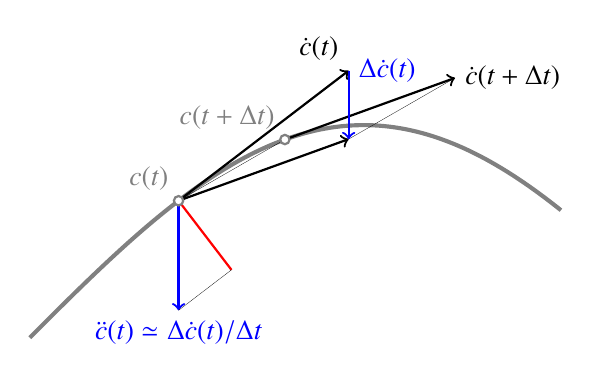
\begin{tikzpicture}[thick,scale=2.7]
\coordinate (O) at (0,0);

\def\deltax{0.5}
\def\vl{0.8}
\def\X{0.7}

\coordinate (A) at ({\X},{sin(180 * \X / 3.14159)});
\coordinate (B) at ({\X + \vl},{sin(180 * \X / 3.14159) + \vl * cos(180 * \X / 3.14159)});

\coordinate (C) at ({\X},{(1-\vl)*sin(180 * \X / 3.14159)});
\coordinate (D) at ({\X+\vl},{sin(180*\X/3.14159) + \vl * cos(180 * (\X + \deltax) / 3.14159)});

\coordinate (E) at ({\X+\deltax},{sin(180 * (\X+\deltax) / 3.14159)});
\coordinate (F) at ({\X + \deltax + \vl}, {sin(180 * (\X + \deltax) / 3.14159) + \vl * cos(180 * (\X + \deltax) / 3.14159)});

\coordinate (G) at ({\X + cos(180 * \X / 3.14159)},{sin(180 * \X / 3.14159)-1});
\coordinate (H) at ({\X + \vl}, {(1-\vl) * sin(180 * \X / 3.14159) + \vl * cos(180 * \X / 3.14159)});

\coordinate (I) at (intersection of A--G and C--H);

\draw[gray,domain=0.0:2.5,line width=1.5,samples=100]
	plot (\x,{sin(180 * \x/3.14159)});

\node at (A) [above left,gray] {$c(t)$};
\node at (E) [above left,gray] {$c(t+\Delta t)$};

\draw[line width=0.1] (A)--(E);
\draw[line width=0.1] (D)--(F);

\draw[->] (A)--(D);
\draw[->] (A)--(B);

\draw[->] (E)--(F);

\draw[->,blue] (B)--(D);

\draw[->,blue] (A)--(C);

\draw[red] (A)--(I);
\draw[line width=0.1] (C)--(I);

\draw[gray,fill=white] (A) circle[radius=0.022] {};
\draw[gray,fill=white] (E) circle[radius=0.022] {};

\node at (B) [above left] {$\dot c(t)$};
\node[blue] at (B) [right] {$\Delta \dot c(t)$};

\node at (F) [right] {$\dot c(t + \Delta t)$};

\node[blue] at (C) [below] {$\ddot c(t)\simeq\Delta\dot c(t)/\Delta t$};

\end{tikzpicture}
\end{document}

